\section{System Overview}
The system shown in \figref{fig:systemoverview} are our current vision for the system.

\begin{figure}[h!]
  \centering
    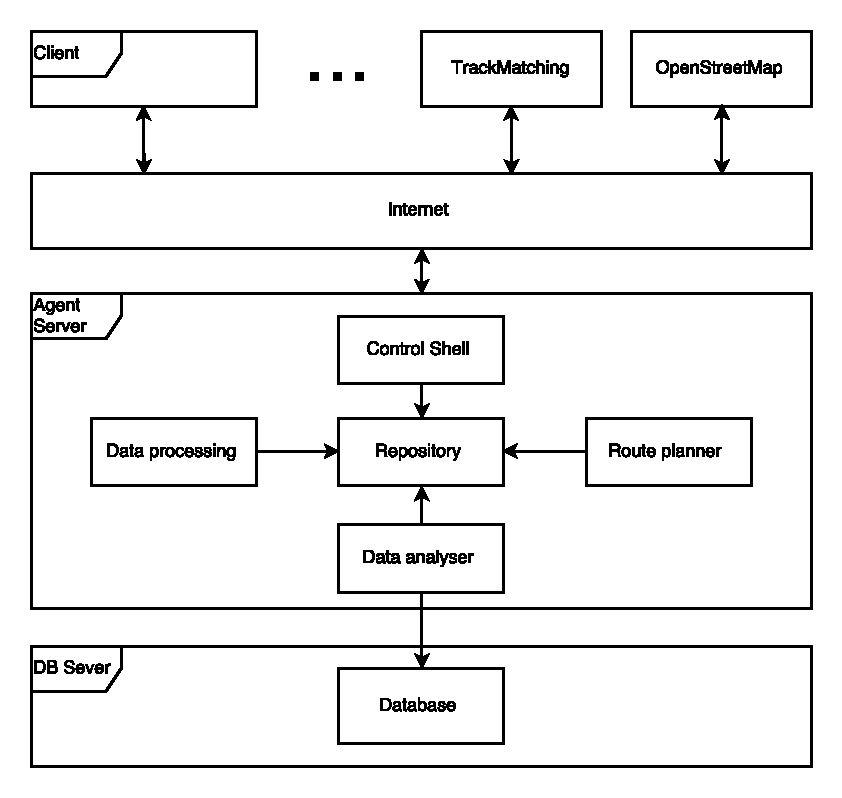
\includegraphics[width=1\textwidth]{figures/architecture.pdf}
    \caption{A course grained system overview.}
    \label{fig:systemoverview}
\end{figure}

The flowschart shows how the user inputs their destination at the start, which sent to a central server together with the source start address. Ther server then uses the data to calculate a route based on the request. The route calculation is based on a initial model of the roadnetwork, such as speedlimits and other restrictions on the roads, and also historical data that have been gathered over time from the users. The route is then sent back to the user, while driving the user will send data back about the drive, this will be the GPS points of the route. This information is then processed and analyzed to check if traffic conditions are as they are supposed to be, and if not the information can be used to recalculate routes for all the drivers which are passing through a that given segment.

So there are 2 processes involved in keeping the data for the map realistic:
\begin{itemize}
	\item Traffic pattern analysis of historical data
	\item Live traffic data analysis
\end{itemize}

The main idea of the traffic pattern analysis is that the data gathered over a given period, at some point will be bulk processed to see if traffic patterns keep the same. Such that the system allways have the best image of the traffic for a particular day, and use these patterns for the best route calculation.

The live traffic data analysis is used check if there are any abnormailties at a given segment, and then being able to propagate this to devices that are going through that segment. Eventually redirecting drivers such that they don't end up at a congested segment, unless nothing else is possible.